\newcommand{\polynomial}[4]{% #1 = x position, y_position, #3 = number of squares, label
	\foreach \j in {0,...,\numexpr#3-1\relax} {
		\draw (#1+\j, #2) rectangle (#1+\j+1, #2+1);
	}
	  \node[anchor=center, inner sep=2pt] (#4) at (#1 + #3/2, #2+0.5) {};
}


\newcommand{\numberedPolynomial}[6]{%
	\pgfmathtruncatemacro{\endj}{#3 - 1}
	\foreach \j in {0,...,\endj} {
		\pgfmathtruncatemacro{\val}{mod(#5 + \j, 4)}
		\pgfmathsetmacro{\xc}{#1+\j+0.5}
		\pgfmathsetmacro{\yc}{#2+0.5}
		\draw (#1+\j, #2) rectangle (#1+\j+1, #2+1);
		\node at (\xc, \yc) {\small \val};
		
		\ifnum#6<0
		% skip drawing
		\else
		\ifnum\j=#6
			\node[draw=red, thick, circle, minimum size=0.8cm, inner sep=0pt] (#4circ) at (\xc, \yc) {};
		\fi
		\fi
	}
	\node[anchor=center, inner sep=2pt] (#4) at (#1 + #3/2, #2+0.5) {};
}



\newcommand{\numberedColoredPolynomial}[6]{%
	\pgfmathtruncatemacro{\endj}{#3 - 1}
	\foreach \j in {0,...,\endj} {
		\pgfmathtruncatemacro{\val}{mod(#5 + \j, 4)}
		\pgfmathsetmacro{\xc}{#1+\j+0.5}
		\pgfmathsetmacro{\yc}{#2+0.5}
		\draw[fill=\mvbcolor, opacity=10] (#1+\j, #2) rectangle (#1+\j+1, #2+1);
		\node at (\xc, \yc) {\small \val};
		
		\ifnum#6<0
		% skip drawing
		\else
		\ifnum\j=#6
			\node[draw=red, thick, circle, minimum size=0.8cm, inner sep=0pt] (#4circ) at (\xc, \yc) {};
		\fi
		\fi
	}
	\node[anchor=center, inner sep=2pt] (#4) at (#1 + #3/2, #2+0.5) {};
}



\newcommand{\coloredPolynomial}[4]{% #1 = x position, y_position, #3 = number of squares, label
	% \definecolor{bitcolorinner}{HTML}{ffa600}
	% \newcommand{\bitcolor}{bitcolorinner}
	\foreach \j in {0,...,\numexpr#3-1\relax} {
		\draw[fill=\mvbcolor, opacity=10] (#1+\j, #2) rectangle (#1+\j+1, #2+1);
	}
	\node[anchor=center, inner sep=2pt] (#4) at (#1 + #3/2, #2+0.5) {};
}

\def\numSquares{5}
\def\spacingPoly{2}


\newcommand{\mvbFigureA}{
	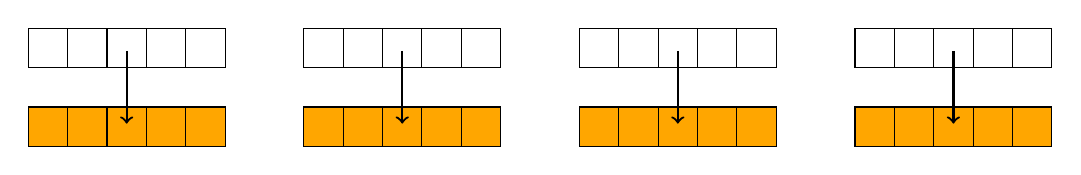
\begin{tikzpicture}[scale=0.5, transform shape]
		\definecolor{mvbcolorinner}{HTML}{ffa600}
		\newcommand{\mvbcolor}{mvbcolorinner}
		
		\foreach \i in {0,...,3} {
			\pgfmathsetmacro{\xpos}{(\numSquares + \spacingPoly) * \i}
			\polynomial{\xpos}{0}{\numSquares}{poly\i}
			
			\coloredPolynomial{\xpos}{-2}{\numSquares}{polyBis\i}
			
			\draw[->, thick] (poly\i.south) -- (polyBis\i.north);
			
			\node[anchor=west] at (\xpos + \numSquares/2, -0.5) {\BlindRotate};
		}
	
	\end{tikzpicture}
}


\newcommand{\mvbFigureB}{
	\begin{tikzpicture}[scale=0.5, transform shape]
		\definecolor{mvbcolorinner}{HTML}{ffa600}
		\newcommand{\mvbcolor}{mvbcolorinner}
		
		\pgfmathsetmacro{\xpos}{(\numSquares + \spacingPoly) * 1.5}
		\polynomial{\xpos}{-4}{\numSquares}{polyBeforeMVB}
		
		\coloredPolynomial{\xpos}{-6}{\numSquares}{polyDuringMVB}
		\draw[->, thick] (polyBeforeMVB.south) -- (polyDuringMVB.north);
		\node[anchor=west] at (\xpos+ \numSquares/2 , -4.5) {\BlindRotate};
		
		\foreach \i in {0,...,3} {
			\pgfmathsetmacro{\xpos}{(\numSquares + \spacingPoly) * \i}
			\coloredPolynomial{\xpos}{-9}{\numSquares}{polyAfterMVB\i}
	
			\draw[->, color=purple, thick] ($(polyDuringMVB.south) + (0, -0.5)$) -- (polyAfterMVB\i.north);
			
			\node[anchor=west] at (\xpos + 1, -7.7) {\huge $\times v_\i$};
		}
	\end{tikzpicture}
}



\newcommand{\treePBSFigure}{%
	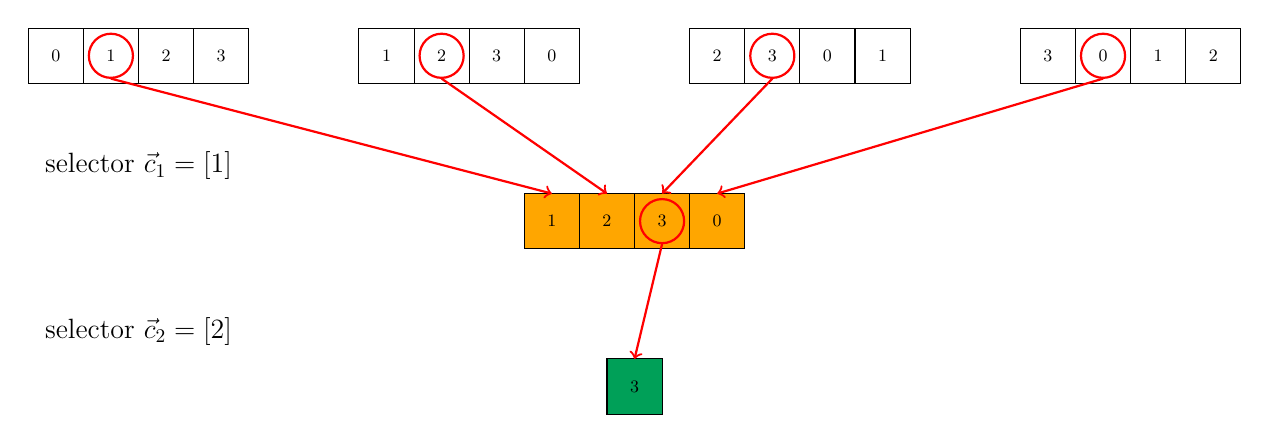
\begin{tikzpicture}[scale=0.7, transform shape]
		\definecolor{mvbcolorinner}{HTML}{ffa600}
		\newcommand{\mvbcolor}{mvbcolorinner}
		
		\definecolor{treecolorinner}{HTML}{00a058}
		\newcommand{\treecolor}{treecolorinner}
		
		\foreach \i in {0,...,3} {
			\pgfmathsetmacro{\xpos}{(\spacingPoly + 4) * \i}
			\numberedPolynomial{\xpos}{0}{4}{polyBeforeTree\i}{\i}{1}
		}
		
		\pgfmathsetmacro{\xpos}{(\spacingPoly + 4) * 1.5}
		\numberedColoredPolynomial{\xpos}{-3}{4}{PolyIntermediate}{1}{2}
		
		\draw[fill=\treecolor, opacity=10] (\xpos+1.5, -6) rectangle (\xpos+2.5, -5);
		
		\node at (\xpos+2, -5.5) {\small 3};
		
		\draw[->, color=red, thick] (polyBeforeTree0circ.south) -- (\xpos + 0.5 ,-2);
		\draw[->, color=red, thick] (polyBeforeTree1circ.south) -- (\xpos + 1.5 ,-2);
		\draw[->, color=red, thick] (polyBeforeTree2circ.south) -- (\xpos + 2.5 ,-2);
		\draw[->, color=red, thick] (polyBeforeTree3circ.south) -- (\xpos + 3.5 ,-2);
		
		\draw[->, color=red, thick] (PolyIntermediatecirc.south) -- (\xpos + 2 ,-5);
		
		\node at (2, -1.5) {\Large selector $\vec c_1 = [1]$};
		\node at (2, -4.5) {\Large selector $\vec c_2 = [2]$};
	\end{tikzpicture}	
}